\chapter{Fazit}
Der Laserscanner, der für die vorliegend implementiert wurde, erfüllt seine Funktion zuverlässig: Innerhalb von wenigen Schritten kann ein Objekt abgetastet und mit einem vertretbaren Messfehler als dreidimensionale Punktewolke dargestellt werden. Auch bei weniger simplen Objekten kann so ein Modell erstellt werden, welches die Charakteristika des Gegenstandes in wiedererkennbarer Weise zuverlässig darstellt. In \ref{fig:figurines} sieht man beispielsweise eine Messung einer kleinen Statuette, welche einem Foto des originalen Objektes gegenübergestellt ist. Das Objekt lässt sich eindeutig wiedererkennen. Der nächste natürliche Schritt in der Verarbeitungspipeline wäre nun die Triangulation der Punktewolke um ein zusammenhängendes Mesh zu erhalten. Dies ist jedoch außerhalb des Zu\-stän\-dig\-keits\-bereichs der vorliegenden Ausarbeitung.\newline
Einige Verbesserung sind für eine Verfeinerung des Verfahrens jedoch denkbar. Zum Einen bietet die Scannerkonstruktion an sich Raum für Verbesserung: Anstatt die gleichmäßige Abtastung der manuellen Einstellung zu überlassen, könnte ein Mechanismus ersannt werden, der es einfacher macht, den Abstand zwischen Aufnahmen genau einzuhalten. Ebenfalls wäre hier die Möglichkeit wünschenswert, kleinere Abstände während der Messung einzuhalten um so eine größere Dichte der Punktewolke zu erhalten. Während eine vollständige Automatisierung hier die beste Lösung darstellt (jedoch den Preis des Laserscanners zugleich erhöhen würde), ist ein Mechanismus wie zum Beispiel eine mechanische Schraube zum Einstellen des Abstandes möglich. Eine andere Erweiterungsmöglichkeit der Scannerkonstruktion stellt die Unterstützung von Messungen von mehr als einer Seite des Objekts dar. Dies würde es möglich machen, das gesamte Objekt als Punktewolke abzubilden, anstatt nur eine Seite. Am Berechnungsanteil des Verfahrens sind alternative Vorgehensweisen an einigen Stellen denkbar. So könnte zum Beispiel bei der Laserlinienerkennung statt mit einem globalen mit einem adaptiven Schwellwert gearbeitet werden. \newline
Auch bei verbleibendem Potential für Verbesserung bietet der implementierte Scanner eine solide Basis zur weiteren Verfeinerung und erfüllt seine Designziele angemessen. Er erlaubt zuverlässige Messungen und demonstriert das Lichtschnittverfahren auf eine praktikable Art und Weise. 

\begin{figure}
\begin{tabular}{cc}
\subfloat[Ansicht Schräg oben]{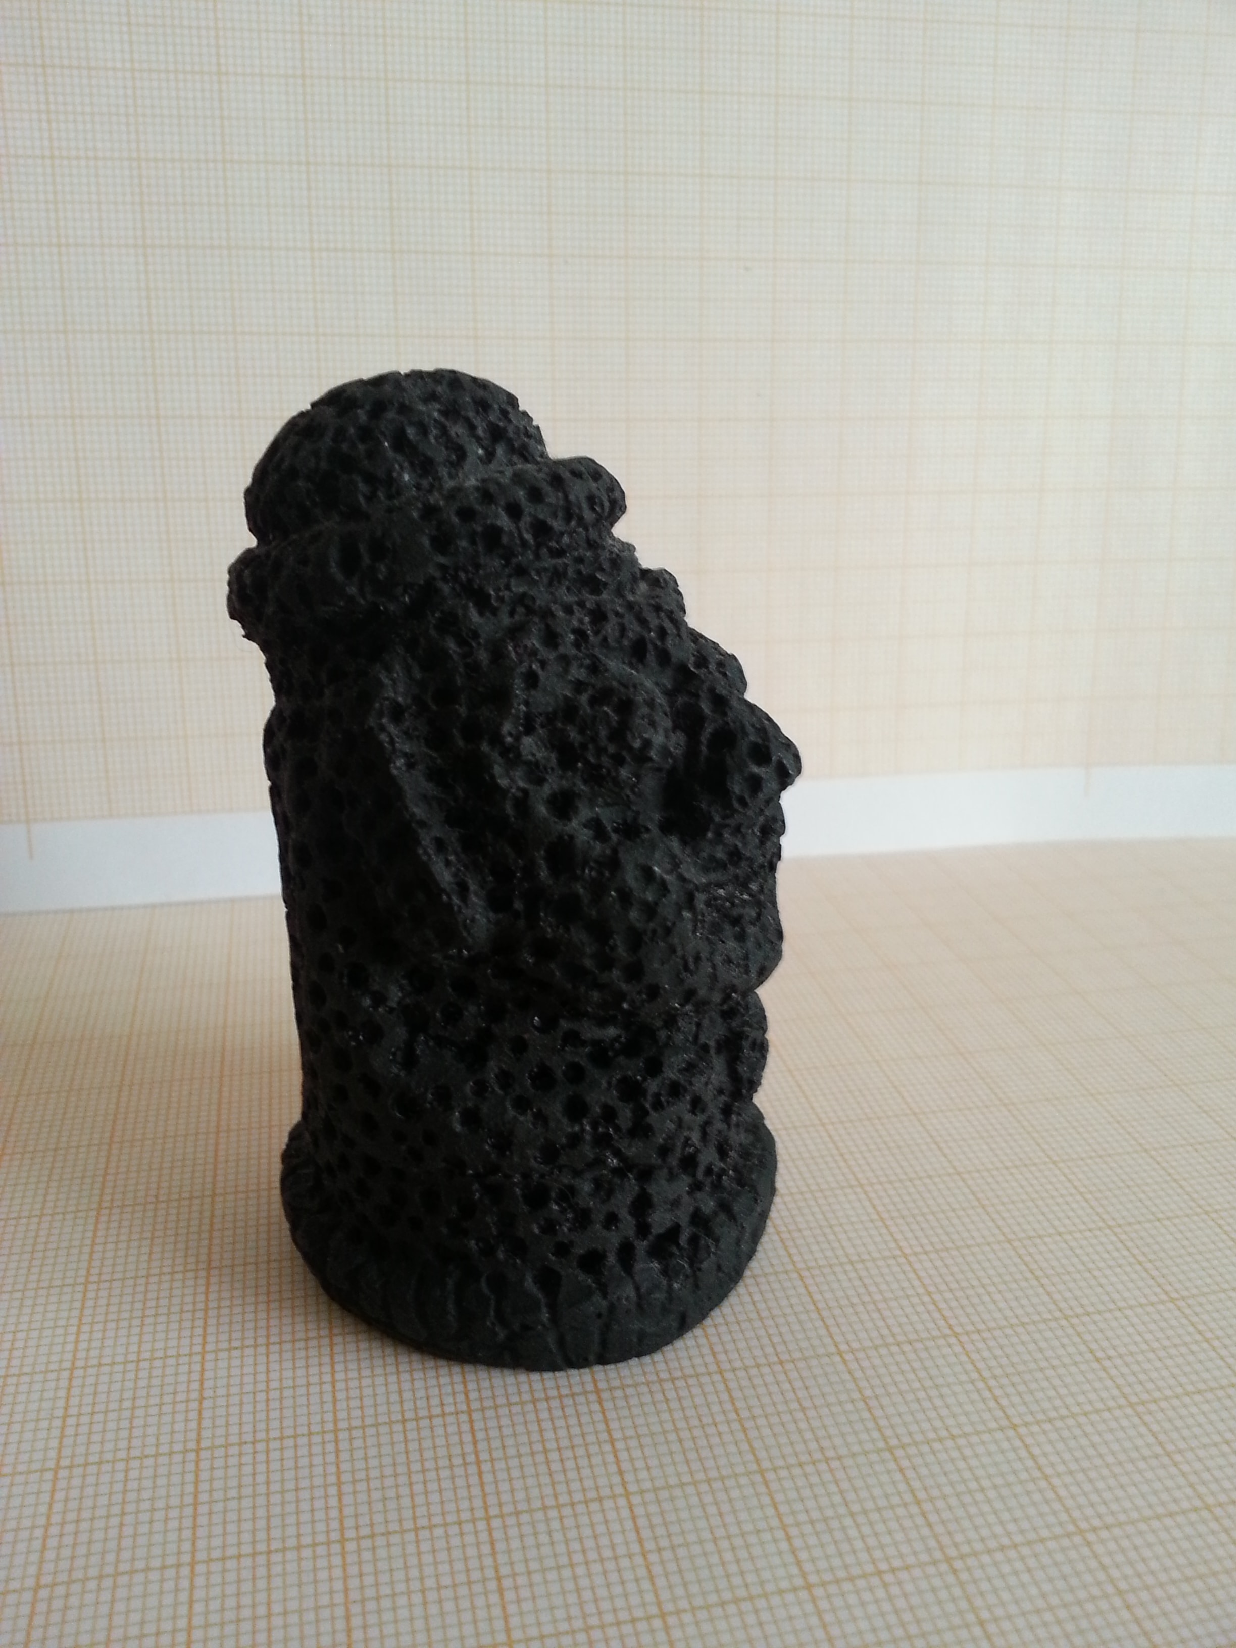
\includegraphics[width = 0.44\textwidth]{images/Figurine2_real.pdf}} &
\subfloat[Ansicht Schräg oben - Messergebnis]{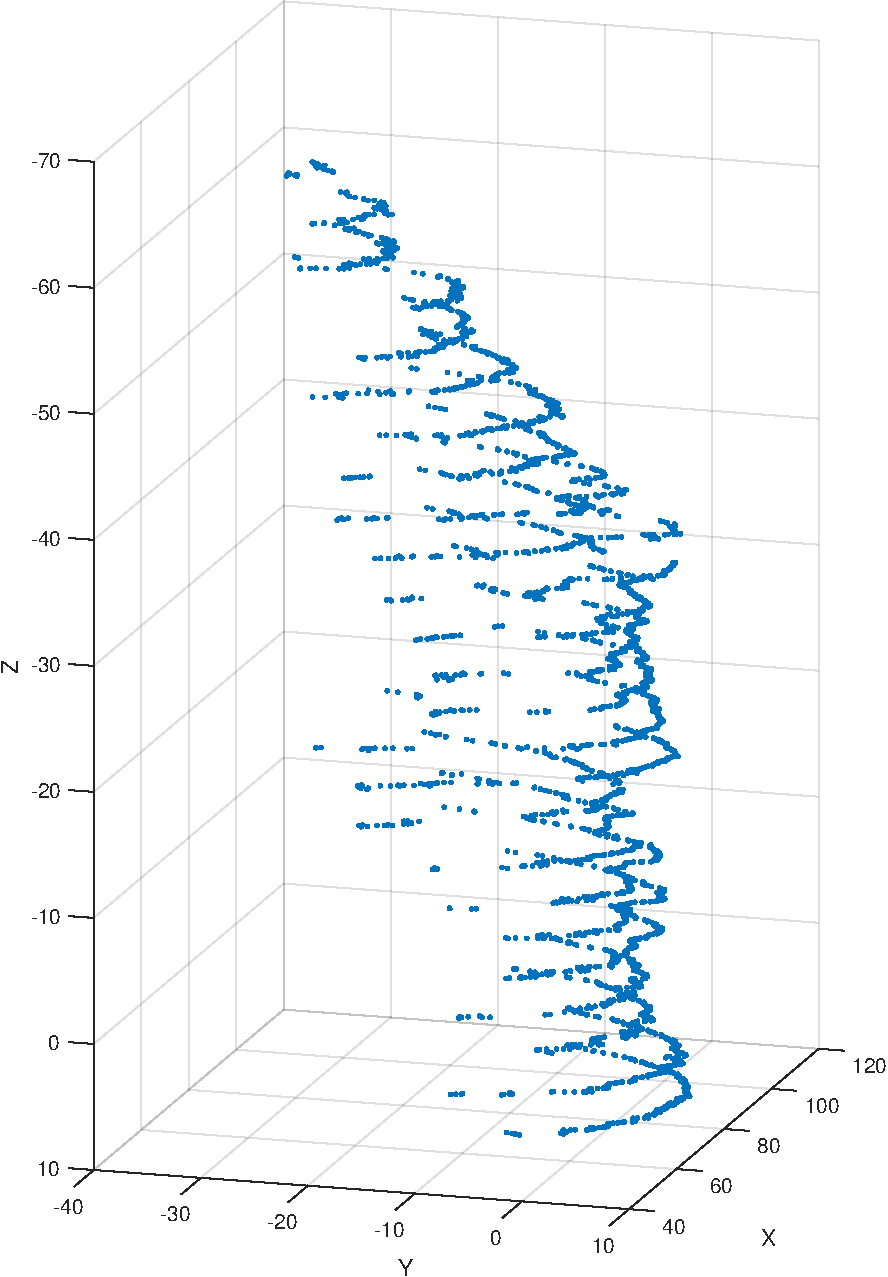
\includegraphics[width = 0.44\textwidth]{images/Figurine2_cropped.pdf}} \\
\subfloat[Ansicht Seite]{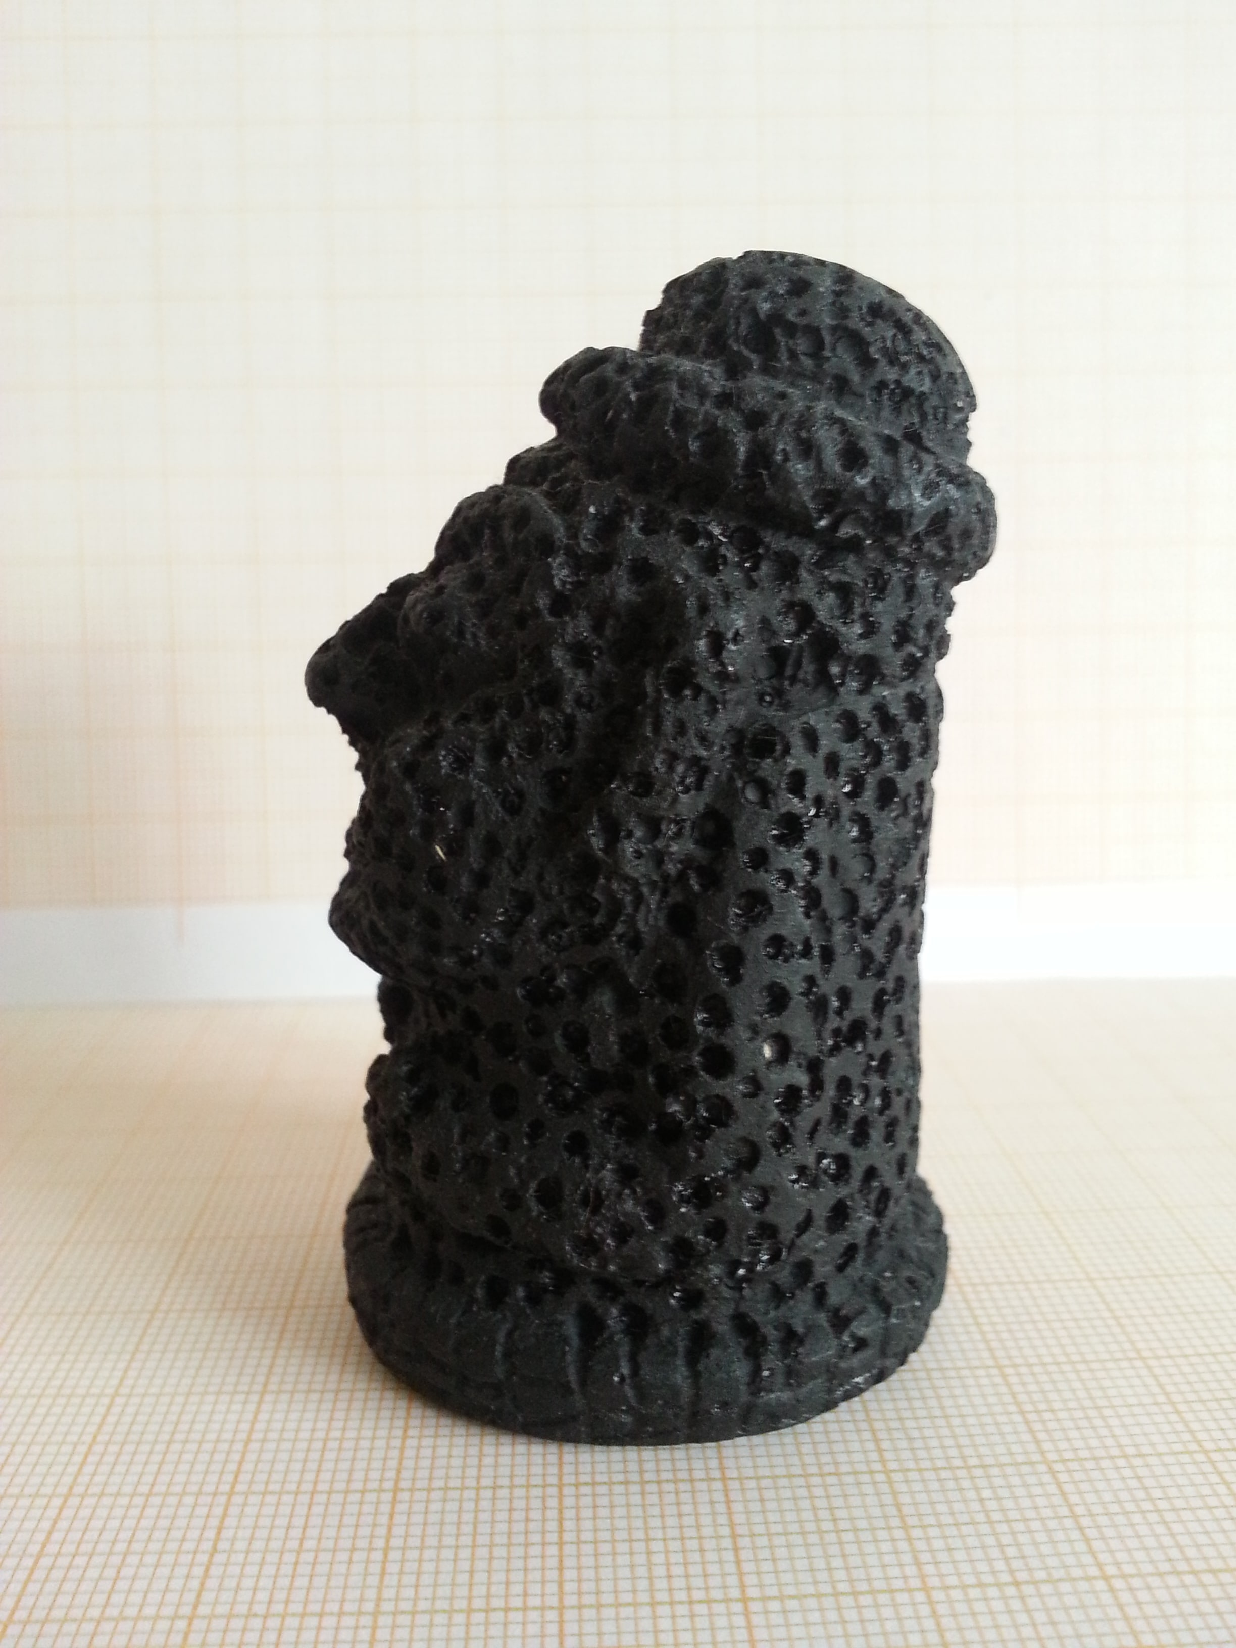
\includegraphics[width = 0.44\textwidth]{images/Figurine1_real.pdf}} &
\subfloat[Ansicht Seite - Messergebnis]{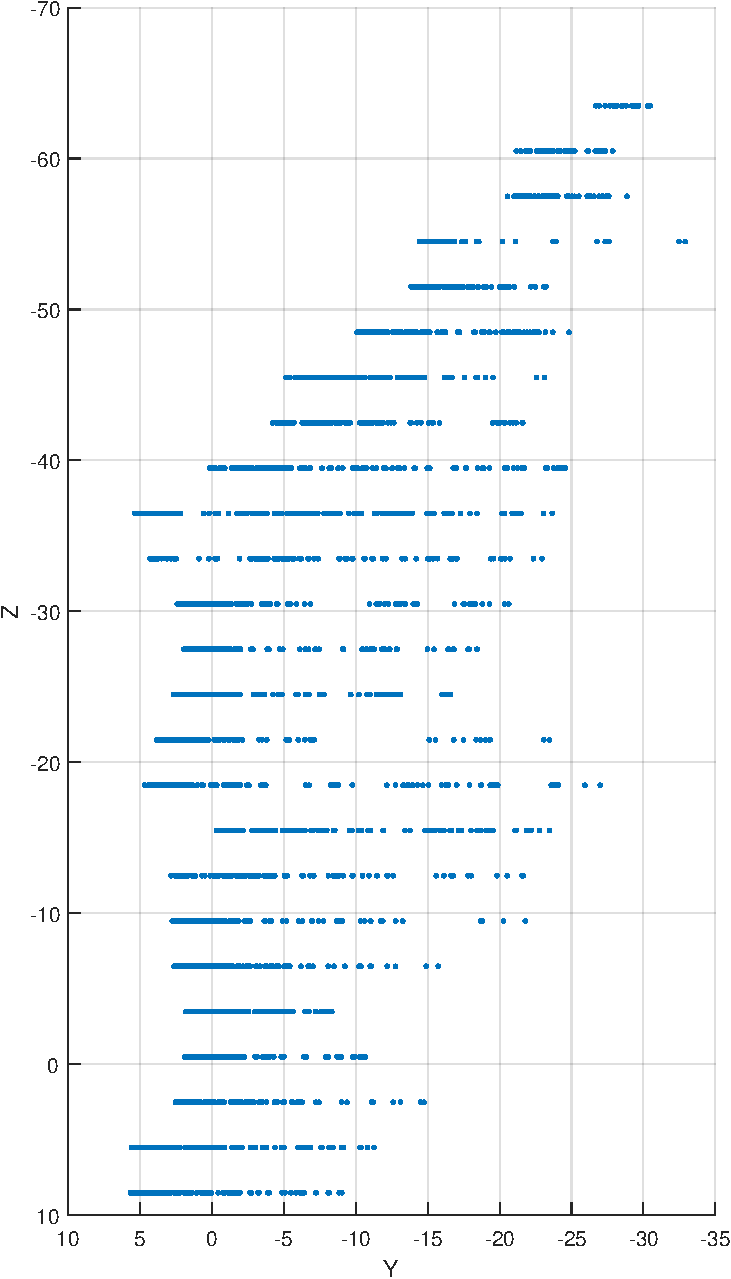
\includegraphics[width = 0.44\textwidth]{images/Figurine1_cropped.pdf}} 
\end{tabular}
\caption{Messergebnisse für ein Objekt mit komplexerer Geometrie aus zwei verschiedenen Blickwinkeln. Das Objekt wurde zwischen je zwei Laserlinienabtastungen mit einem Abstand von 3mm vermessen, was es bereits erlaubt die Objektsilhouette zu erkennen. Die Diskrepanz, dass einige vermessene Punkte auf der Z-Achse im positiven Bereich liegen, wird auf Ungenauigkeiten bei der Kamerakalibrierung und den Bedingungen während des Vermessungsvorgangs zurückgeführt.}\label{fig:figurines}
\end{figure}